\section{Experiments}
\label{sec:exp}
To evaluate the effectiveness and robustness of SWaST, we conducted a series of experiments. All results reported in the tables are averaged over 5 runs. 
We first briefly review the experimental setup, followed by specific results. Detailed method descriptions and additional results with other pruning/coreset methods, can be found in the Appendix.

\begin{itemize}
    \item \textbf{Datasets and network architectures:} We conduct experiments on CIFAR-10/100 \cite{krizhevsky2009cifar}, TinyImageNet~\cite{le2015tiny}, and ImageNet-1K~\cite{deng2009imagenet} datasets, using ResNet-18 and ResNet-101 to verify our method's effectiveness across different model scales.  
    \item \textbf{Coreset selection and pruning methods:} Given the varying scales of datasets, we adopt selection methods with different computational complexities: GradMatch~\cite{killamsetty2021grad} for CIFAR, Moderate~\cite{xia2022moderate} for TinyImageNet, and EL2N~\cite{paul2021deep} for ImageNet-1K. We employ the RigL~\cite{evci2020rigging} method as our default pruning algorithm.
    \item \textbf{Pruning configuration:} For SWaST-trim, the pruning rate applies to FC layers; for SWaST-cut, it applies to the backbone with FC layers fixed at 90\% pruning. Configuration details are provided in the Appendix. Detailed analysis and justification for these configuration choices are provided in the Appendix.
    \item \textbf{Evaluation on datasets with label noise: } To thoroughly analyze the synergistic effects between weight pruning and coreset selection, we introduce label noise into the datasets in certain experiments.
\end{itemize}

\begin{figure}[!t]
  \centering
  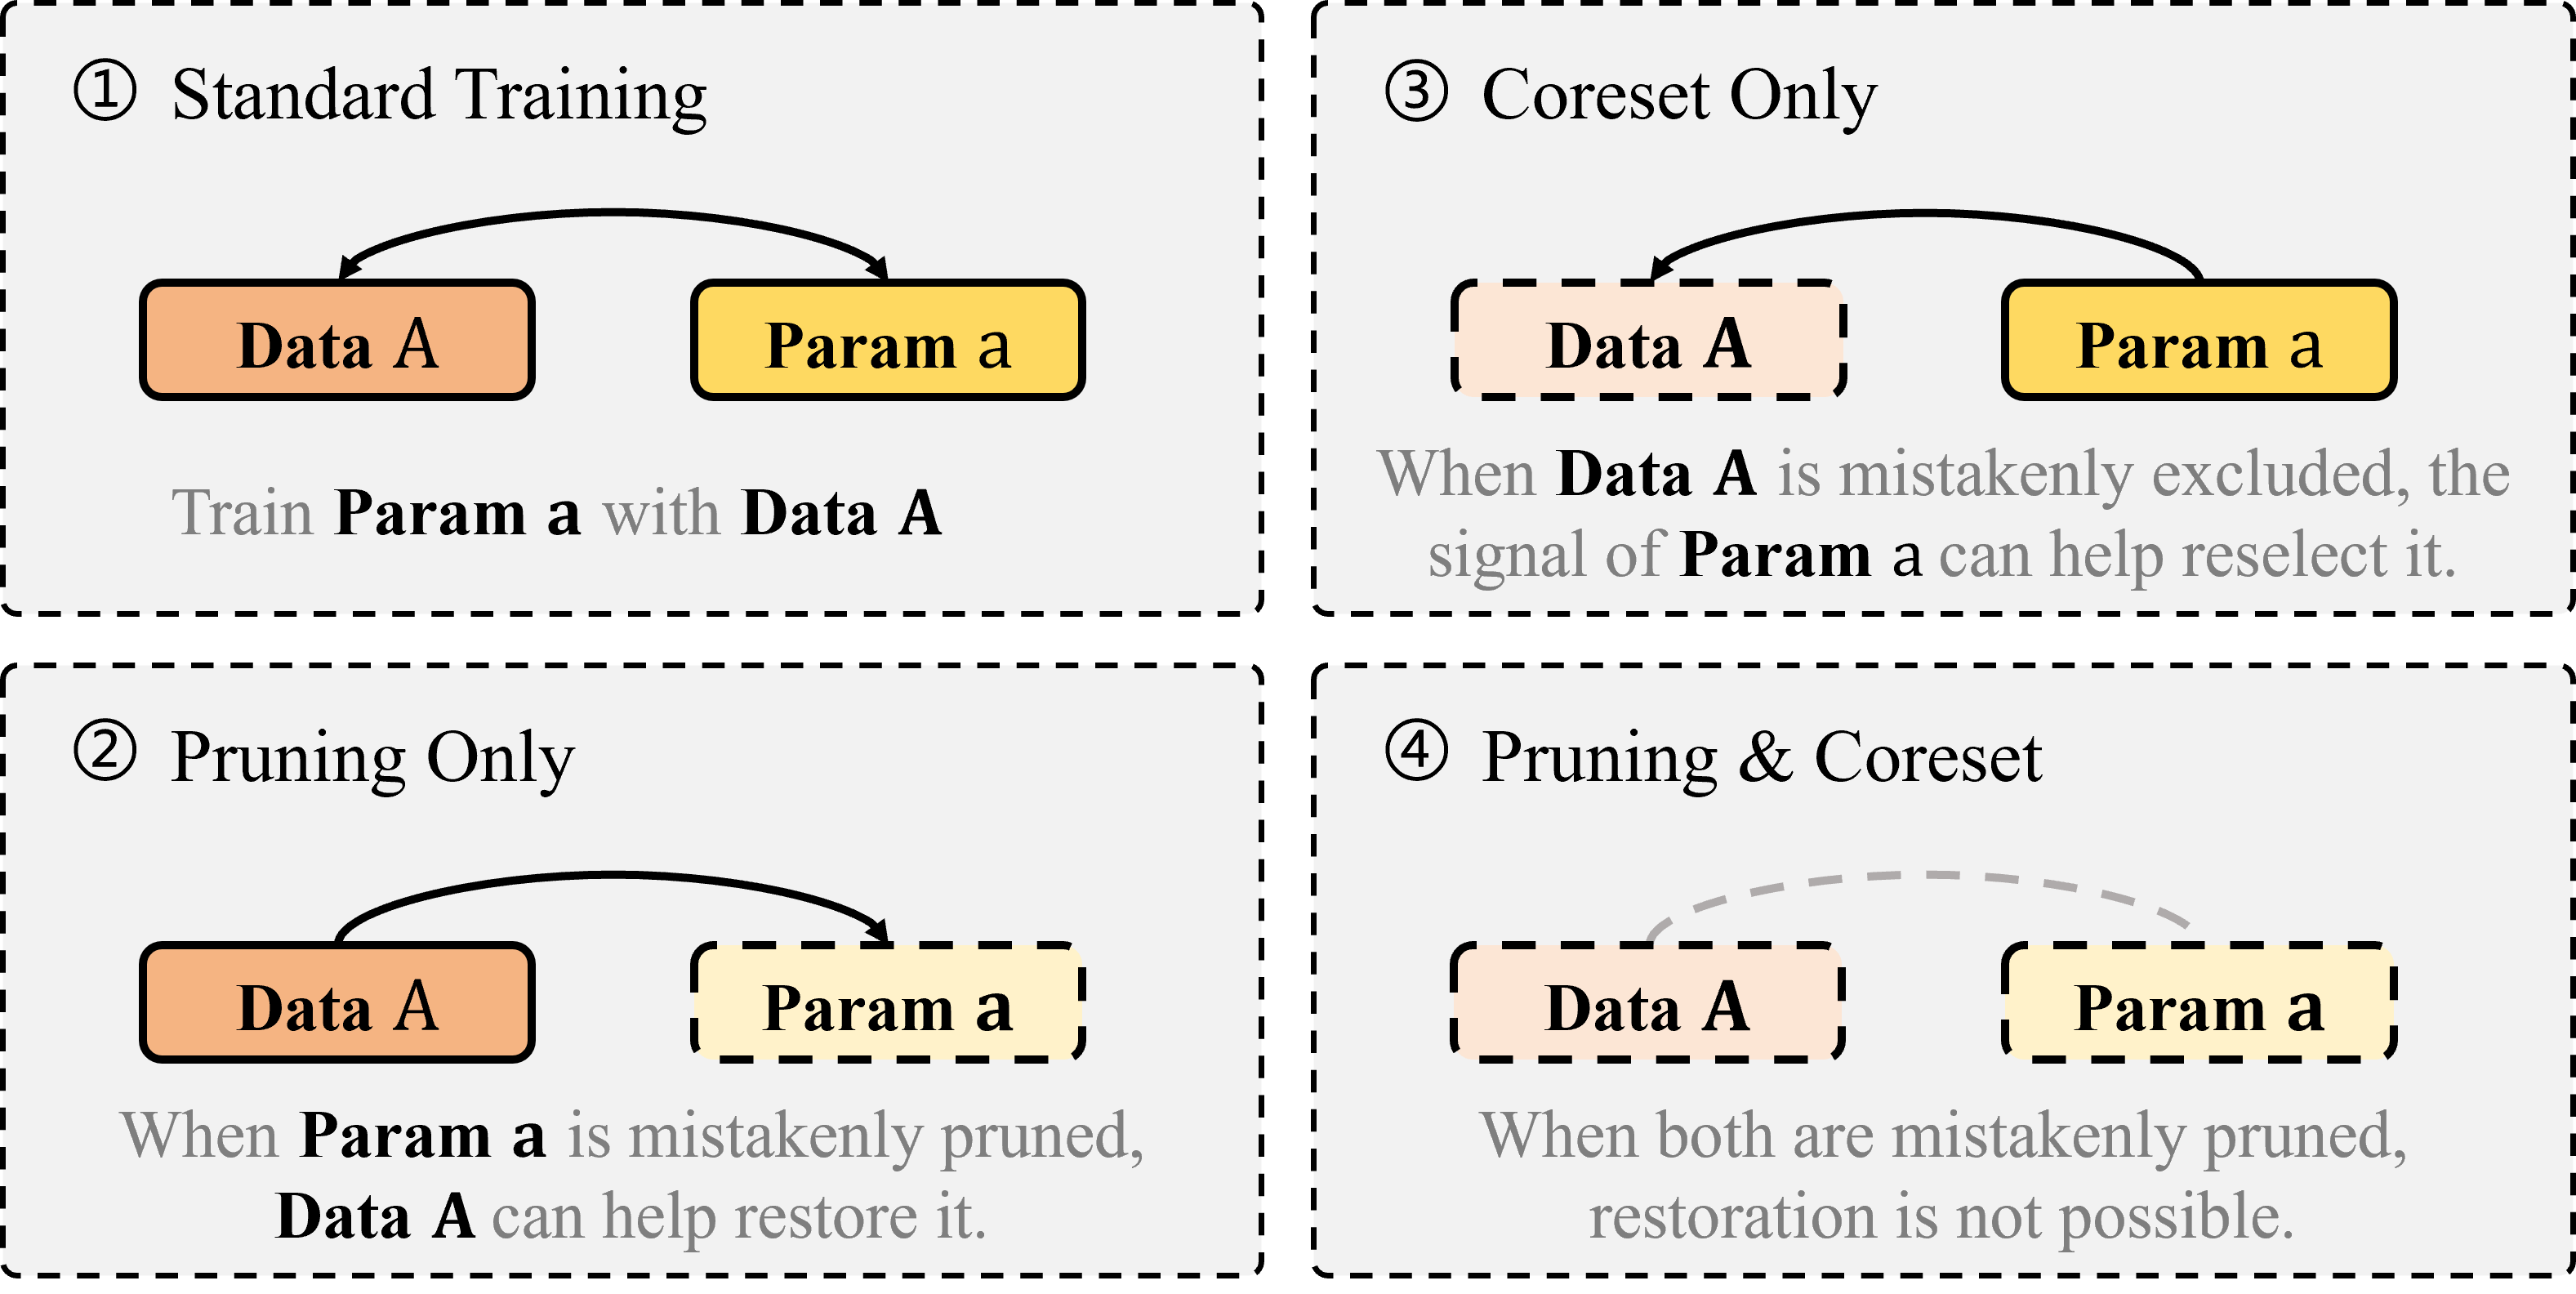
\includegraphics[width=1.0\linewidth]{figs/double-loss.png}
   \caption{Illustration of the “critical double-loss" phenomenon in concurrent weight pruning and sample tailoring: (1) Standard Training shows the close link between Data $A$ and Param $a$. (2) Pruning Only allows recovery of Param $a$ using Data $A$ when mistakenly pruned. (3) Coreset Only supports re-selection of Data $A$ through Param $a$ when excluded in error. (4) Pruning \& Coreset causes irreversible degradation from simultaneous exclusion.}
   \label{fig:double-loss}
\end{figure}

\subsection{Main Results}
\label{sec:4-1}

\paragraph{Efficiency analysis.} 
\begin{figure}[!b]
  \centering
  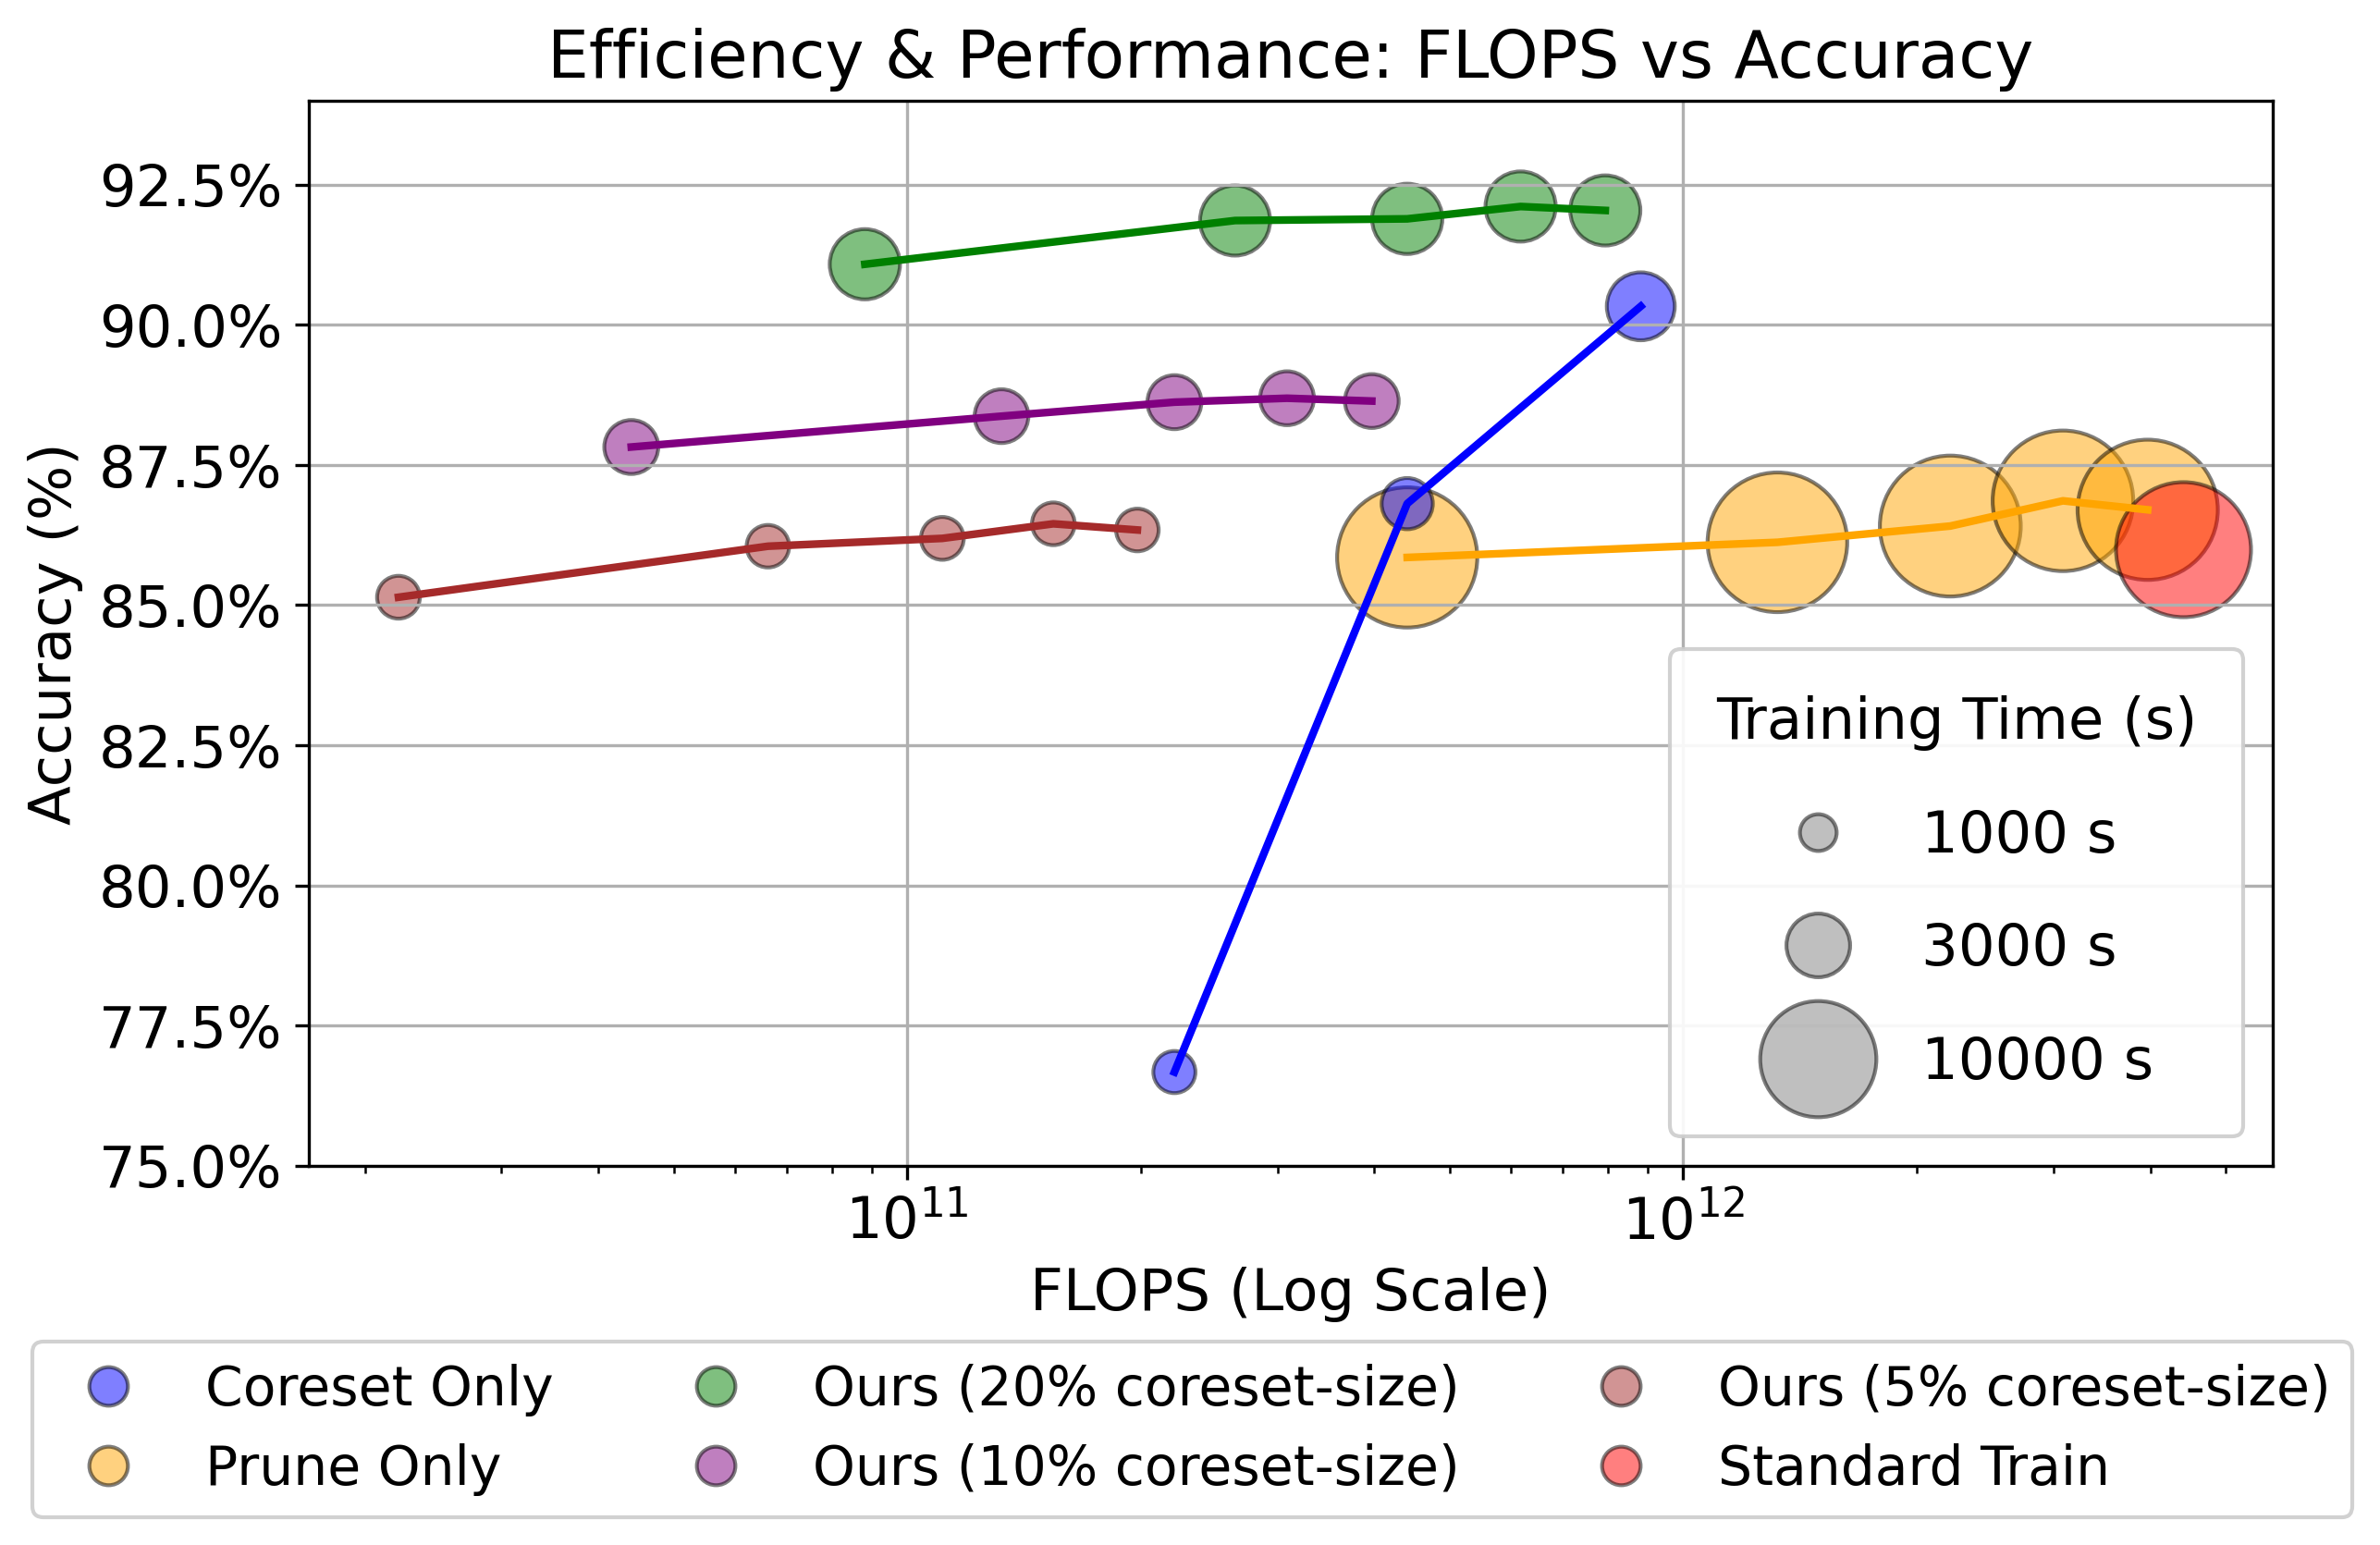
\includegraphics[width=1.0\linewidth]{figs/flops_acc_aaai.png}
   \caption{Efficiency vs.\ accuracy trade-offs (bubble area \(\propto\) training time), where the upper-left region indicates optimal performance (high accuracy with low FLOPs).}
   \label{fig:efficiency}
\end{figure}
\label{sec:efficiency_analysis}  

\begin{table*}[!t] 
    \centering  
    \resizebox{\textwidth}{!}{  
    \renewcommand{\arraystretch}{1.2}
    \begin{tabular}{lcccccccc}  
    \hline
    &  &  & \multicolumn{5}{c}{\textbf{SWaST-trim with different Prune Rate}} &  \\ \cline{4-8}  
    \multirow{-2}{*}{\textbf{Model}} & \multirow{-2}{*}{\textbf{Dataset}} & \multirow{-2}{*}{\textbf{Coreset Size}} & 90\% & 70\% & 50\% & 30\% & 10\% & \multirow{-2}{*}{\textbf{Coreset-only}} \\ \hline  
    &  & 10\% & {\color{red}$92.58_{{\tiny(+0.38)}}$} & {\color{blue}$92.53_{{\tiny(+0.33)}}$} & {\color{blue}$92.40_{{\tiny(+0.20)}}$} & $92.32_{{\tiny(+0.12)}}$ & $92.29_{{\tiny(+0.09)}}$ & 92.20 \\
    &  & 5\% & {\color{red}$90.16_{{\tiny(+0.49)}}$} & {\color{blue}$90.07_{{\tiny(+0.40)}}$} & {\color{blue}\textbf{$89.92_{{\tiny(+0.25)}}$}} & $89.81_{{\tiny(+0.14)}}$ & $89.77_{{\tiny(+0.10)}}$ & 89.67 \\
    & \multirow{-3}{*}{CIFAR-10} & 1\% & {\color{red}$78.60_{{\tiny(+2.97)}}$} & {\color{blue}$78.33_{{\tiny(+2.80)}}$} & {\color{blue}$77.14_{{\tiny(+1.61)}}$} & \textbf{$76.26_{{\tiny(+0.73)}}$} & $76.01_{{\tiny(+0.48)}}$ & 75.53 \\ \cline{2-9}   
    &  & 10\% & {\color{red}$71.94_{{\tiny(+0.97)}}$} & {\color{blue}$71.76_{{\tiny(+0.79)}}$} & {\color{blue}$71.44_{{\tiny(+0.47)}}$} & \textbf{$71.27_{{\tiny(+0.30)}}$} & $71.20_{{\tiny(+0.23)}}$ & 70.97 \\
    &  & 5\% & {\color{red}$66.19_{{\tiny(+1.40)}}$} & {\color{blue}$65.97_{{\tiny(+1.18)}}$} & {\color{blue}$65.56_{{\tiny(+0.77)}}$} & $65.22_{{\tiny(+0.43)}}$ & \textbf{$65.09_{{\tiny(+0.30)}}$} & 64.79 \\
    \multirow{-6}{*}{ResNet-18} & \multirow{-3}{*}{CIFAR-100} & 1\% & {\color{red}$38.38_{{\tiny(+1.96')}}$} & {\color{blue}$38.12_{{\tiny(+1.70)}}$} & {\color{blue}\textbf{$37.58_{{\tiny(+1.16)}}$}} & $37.01_{{\tiny(+0.59)}}$ & $36.88_{{\tiny(+0.46)}}$ & 36.42 \\ \hline  
    \multicolumn{1}{c}{} &  & 10\% & {\color{red}$92.60_{{\tiny(+1.47)}}$} & {\color{blue}$92.45_{{\tiny(+1.32)}}$} & {\color{blue}$92.12_{{\tiny(+0.99)}}$} & $91.89_{{\tiny(+0.76)}}$ & $91.54_{{\tiny(+0.41)}}$ & 91.13 \\
    \multicolumn{1}{c}{} &  & 5\% & {\color{red}$89.81_{{\tiny(+3.53)}}$} & {\color{blue}$89.39_{{\tiny(+3.11)}}$} & {\color{blue}$88.04_{{\tiny(+1.76)}}$} & $87.46_{{\tiny(+1.18)}}$ & $87.29_{{\tiny(+1.01)}}$ & 86.28 \\
    \multicolumn{1}{c}{} & \multirow{-3}{*}{CIFAR-10} & 1\% & {\color{red}$66.23_{{\tiny(+16.51)}}$} & {\color{blue}$63.36_{{\tiny(+13.64)}}$} & {\color{blue}$60.46_{{\tiny(+10.74)}}$} & $55.45_{{\tiny(+5.73)}}$ & $53.02_{{\tiny(+3.30)}}$ & 49.72 \\ \cline{2-9}   
    \multicolumn{1}{c}{} &  & 10\% & {\color{red}$71.93_{{\tiny(+3.14)}}$} & {\color{blue}$71.68_{{\tiny(+2.89)}}$} & {\color{blue}$70.47_{{\tiny(+1.68)}}$} & $70.01_{{\tiny(+1.22)}}$ & $68.74_{{\tiny(+0.95)}}$ & 68.79 \\
    \multicolumn{1}{c}{} &  & 5\% & {\color{red}$61.72_{{\tiny(+7.84)}}$} & {\color{blue}$60.25_{{\tiny(+6.37)}}$} & {\color{blue}$58.19_{{\tiny(+4.31)}}$} & $56.63_{{\tiny(+2.75)}}$ & $55.82_{{\tiny(+1.94)}}$ & 53.88 \\
    \multirow{-6}{*}{ResNet-101} & \multirow{-3}{*}{CIFAR-100} & 1\% & {\color{red}$21.16_{{\tiny(+9.47)}}$} & {\color{blue}$18.53_{{\tiny(+6.84)}}$} & {\color{blue}\textbf{$16.04_{{\tiny(+4.35)}}$}} & $14.46_{{\tiny(+2.77)}}$ & $13.87_{{\tiny(+2.18)}}$ & 11.69 \\ \hline
    &  &  & \multicolumn{5}{c}{\textbf{SWaST-cut with different Prune Rate}} &  \\ \cline{4-8}  
    \multirow{-2}{*}{\textbf{Model}} & \multirow{-2}{*}{\textbf{Dataset}} & \multirow{-2}{*}{\textbf{Coreset Size}} & 90\% & 70\% & 50\% & 30\% & 10\% & \multirow{-2}{*}{\textbf{Coreset-only}} \\ \hline  
    &  & 10\% & $91.53_{{\tiny(-0.67)}}$ & $92.32_{{\tiny(+0.12)}}$ & {\color{blue}$92.40_{{\tiny(+0.20)}}$} & {\color{red}\textbf{$92.92_{{\tiny(+0.72)}}$}} & {\color{blue}$92.60_{{\tiny(+0.40)}}$} & 92.20 \\
    &  & 5\% & $89.32_{{\tiny(-0.35)}}$ & $90.12_{{\tiny(+0.45)}}$ & {\color{blue}\textbf{$90.35_{{\tiny(+0.68)}}$}} & {\color{red}$91.11_{{\tiny(+1.44)}}$} & {\color{blue}$90.18_{{\tiny(+0.51)}}$} & 89.67 \\
    & \multirow{-3}{*}{CIFAR-10} & 1\% & $77.13_{{\tiny(+1.60)}}$ & $78.52_{{\tiny(+2.99)}}$ & {\color{blue}$78.57_{{\tiny(+3.24)}}$} & {\color{red}\textbf{$78.70_{{\tiny(+3.17)}}$}} & {\color{blue}$78.67_{{\tiny(+3.14)}}$} & 75.53 \\ \cline{2-9}   
    &  & 10\% & $67.98_{{\tiny(-2.99)}}$ & $71.09_{{\tiny(+0.12)}}$ & {\color{blue}$71.91_{{\tiny(+0.94)}}$} & {\color{red}\textbf{$72.09_{{\tiny(+1.12)}}$}} & {\color{blue}$71.99_{{\tiny(+1.02)}}$} & 70.97 \\
    &  & 5\% & $63.24_{{\tiny(-1.55)}}$ & $65.15_{{\tiny(+0.36)}}$ & {\color{blue}$65.55_{{\tiny(+0.76)}}$} & {\color{red}$66.81_{{\tiny(+2.02)}}$} & {\color{blue}\textbf{$66.30_{{\tiny(+1.51)}}$}} & 64.79 \\
    \multirow{-6}{*}{ResNet-18} & \multirow{-3}{*}{CIFAR-100} & 1\% & $35.80_{{\tiny(-0.62)}}$ & $37.81_{{\tiny(+1.39)}}$ & {\color{red}\textbf{$40.29_{{\tiny(+3.87)}}$}} & {\color{blue}$39.55_{{\tiny(+3.13)}}$} & {\color{blue}$38.53_{{\tiny(+2.11)}}$} & 36.42 \\ \hline
    \multicolumn{3}{c}{\textbf{Params. After Pruning}} & 1.2M & 3.5M & 5.8M & 8.2M & 10.5M & 11.7M \\ \hline
    
    \multicolumn{1}{c}{} &  & 10\% & $91.85_{{\tiny(+0.72)}}$ & $92.46_{{\tiny(+1.33)}}$ & {\color{blue}$92.61_{{\tiny(+1.48)}}$} & {\color{red}\textbf{$92.96_{{\tiny(+1.83)}}$}} & {\color{blue}$92.62_{{\tiny(+1.49)}}$} & 91.13 \\
    \multicolumn{1}{c}{} &  & 5\% & $88.90_{{\tiny(+2.62)}}$ & $89.55_{{\tiny(+3.27)}}$ & {\color{blue}$90.00_{{\tiny(+3.72)}}$} & {\color{red}\textbf{$90.13_{{\tiny(+3.85)}}$}} & {\color{blue}$89.99_{{\tiny(+3.71)}}$} & 86.28 \\
    \multicolumn{1}{c}{} & \multirow{-3}{*}{CIFAR-10} & 1\% & $64.57_{{\tiny(+14.85)}}$ & $64.82_{{\tiny(+15.10)}}$ & {\color{blue}$66.92_{{\tiny(+17.20)}}$} & {\color{red}\textbf{$67.55_{{\tiny(+17.83)}}$}} & {\color{blue}$66.52_{{\tiny(+16.80)}}$}  & 49.72 \\ \cline{2-9}   
    \multicolumn{1}{c}{} &  & 10\% & $69.41_{{\tiny(+0.62)}}$ & $70.73_{{\tiny(+1.94)}}$ & {\color{blue}$71.75_{{\tiny(+2.96)}}$} & {\color{blue}$71.95_{{\tiny(+3.16)}}$} & {\color{red}\textbf{$72.05_{{\tiny(+3.26)}}$}} & 68.79 \\
    \multicolumn{1}{c}{} &  & 5\% & $59.27_{{\tiny(+5.39)}}$ & $59.65_{{\tiny(+5.77)}}$ & {\color{blue}$62.87_{{\tiny(+8.99)}}$} & {\color{red}\textbf{$62.97_{{\tiny(+9.09)}}$}} & {\color{blue}$62.14_{{\tiny(+8.26)}}$} & 53.88 \\
    & \multirow{-3}{*}{CIFAR-100} & 1\% & $19.17_{{\tiny(+7.48)}}$ & $20.11_{{\tiny(+8.42)}}$ & {\color{red}\textbf{$21.24_{{\tiny(+9.55)}}$}} & {\color{blue}$20.99_{{\tiny(+9.30)}}$} & {\color{blue}$21.19_{{\tiny(+9.50)}}$} & 11.69 \\ \cline{2-9}
    &  & 10\% & $51.29_{{\tiny(+2.63)}}$ & $52.78_{{\tiny(+4.12)}}$ & {\color{red}$53.49_{{\tiny(+4.83)}}$} & {\color{blue}$53.14_{{\tiny(+4.48)}}$} & {\color{blue}$52.98_{{\tiny(+4.32)}}$} & 48.66 \\
     & \multirow{-2}{*}{TinyImageNet} & 5\% & $38.65_{{\tiny(+3.55)}}$ & {\color{blue}$42.83_{{\tiny(+7.73)}}$} & {\color{red}$42.93_{{\tiny(+7.83)}}$} & {\color{blue}$41.94_{{\tiny(+6.84)}}$} & $41.21_{{\tiny(+6.11)}}$ & 35.10 \\ \cline{2-9}
    &  & 10\% & $37.55_{{\tiny(+5.83)}}$ & $38.28_{{\tiny(+6.56)}}$ & {\color{blue}$38.92_{{\tiny(+7.20)}}$} & {\color{blue}$39.19_{{\tiny(+7.47)}}$} & {\color{red}$39.47_{{\tiny(+7.75)}}$} & 31.72 \\
    \multirow{-10}{*}{ResNet-101} & \multirow{-2}{*}{ImageNet-1k} & 5\% & $31.63_{{\tiny(+1.35)}}$ & $32.25_{{\tiny(+1.97)}}$ & {\color{blue}$32.71_{{\tiny(+2.43)}}$} & {\color{red}$34.34_{{\tiny(+4.06)}}$} & {\color{blue}$33.12_{{\tiny(+2.84)}}$} & 30.28 \\ \hline
    \multicolumn{3}{c}{\textbf{Params. After Pruning}} & 4.5M & 13.3M & 22.3M & 31.2M & 40.1M & 44.5M \\ \hline
    \end{tabular}} 
    \caption{Comparison for various pruning rates and subset fractions on different datasets. Values in parentheses show differences from the Coreset-only baseline. {\color{red}Red}/{\color{blue}blue} numbers indicate best and runner-up results within each row.  SWaST-trim (upper half) prunes only FC layers, maintaining parameters near originals: $\sim$11.2M--11.7M for ResNet-18 (original 11.7M) and $\sim$42.7M--44.5M for ResNet-101 (original 44.5M). SWaST-cut (lower half) applies global pruning with explicit parameter counts listed.  \textbf{Row-wise}: Both SWaST variants consistently outperform the baseline, with gains up to \textbf{17.83\%}. 
    \textbf{Column-wise}: Performance improvements \textbf{increase as coreset sizes decrease} since smaller coresets present greater selection challenge and higher overfitting risk, while weight
    pruning mitigates these issues.
    }
    \label{tab:tab1}
\end{table*}

To validate the efficiency of SWaST, we present experimental results conducted on ResNet101, as illustrated in Fig.~\ref{fig:efficiency}. In this visualization, the x-axis represents FLOPS, the y-axis shows accuracy, and the circle sizes indicate training time (detailed experimental configurations and settings are provided in the appendix). As observed from the results, our method achieves significantly higher accuracy compared to other approaches under equivalent FLOPS constraints, demonstrating superior computational efficiency.

\paragraph{Weight pruning improves coreset selection.}
Following the protocol established in~\cite{killamsetty2021grad},  we benchmark our proposed methods (SWaST-trim and SWaST-cut) against the coreset-only baseline. Table~\ref{tab:tab1} demonstrates that SWaST variants exhibit two key advantages when operating with identical subset sizes:
\begin{figure*}[!htbp]
  \centering
  \begin{subfigure}{0.32\linewidth}
    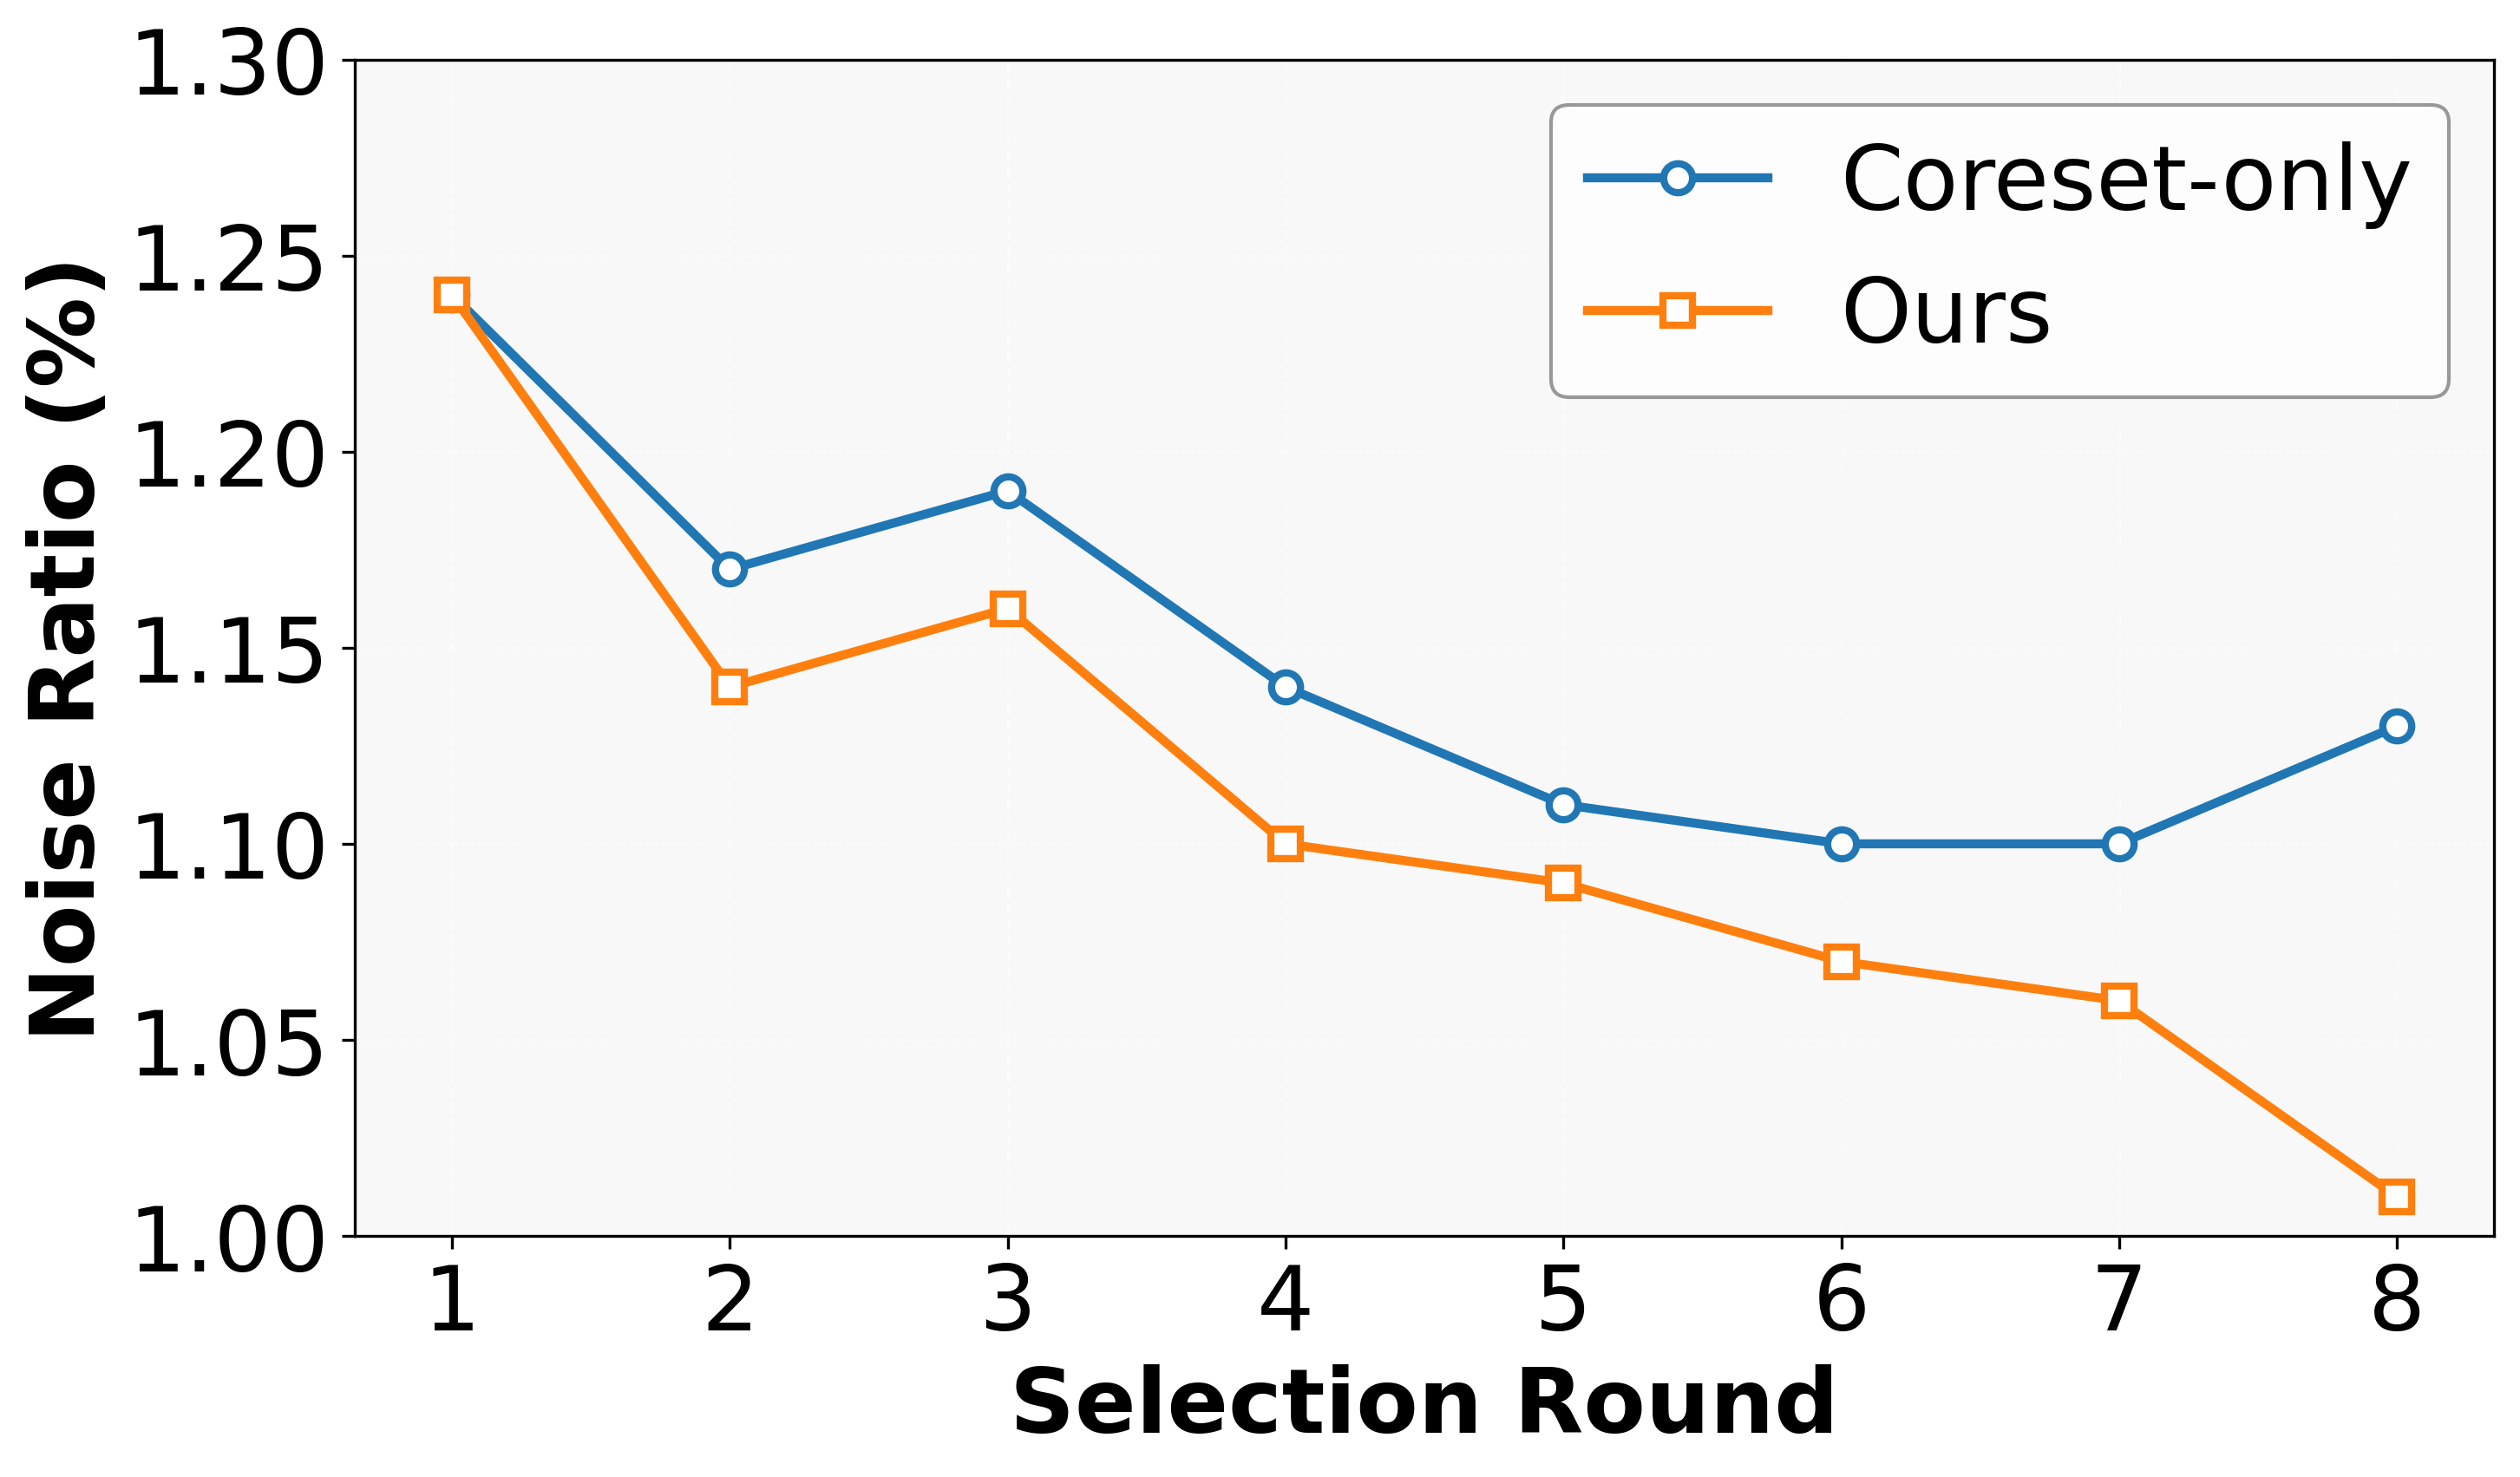
\includegraphics[width=1.0\linewidth]{figs/noise_ratio.png}
    \caption{Noise in selected coresets}
    \label{fig:noise_ratio}
  \end{subfigure}
  \hfill
  \begin{subfigure}{0.32\linewidth}
    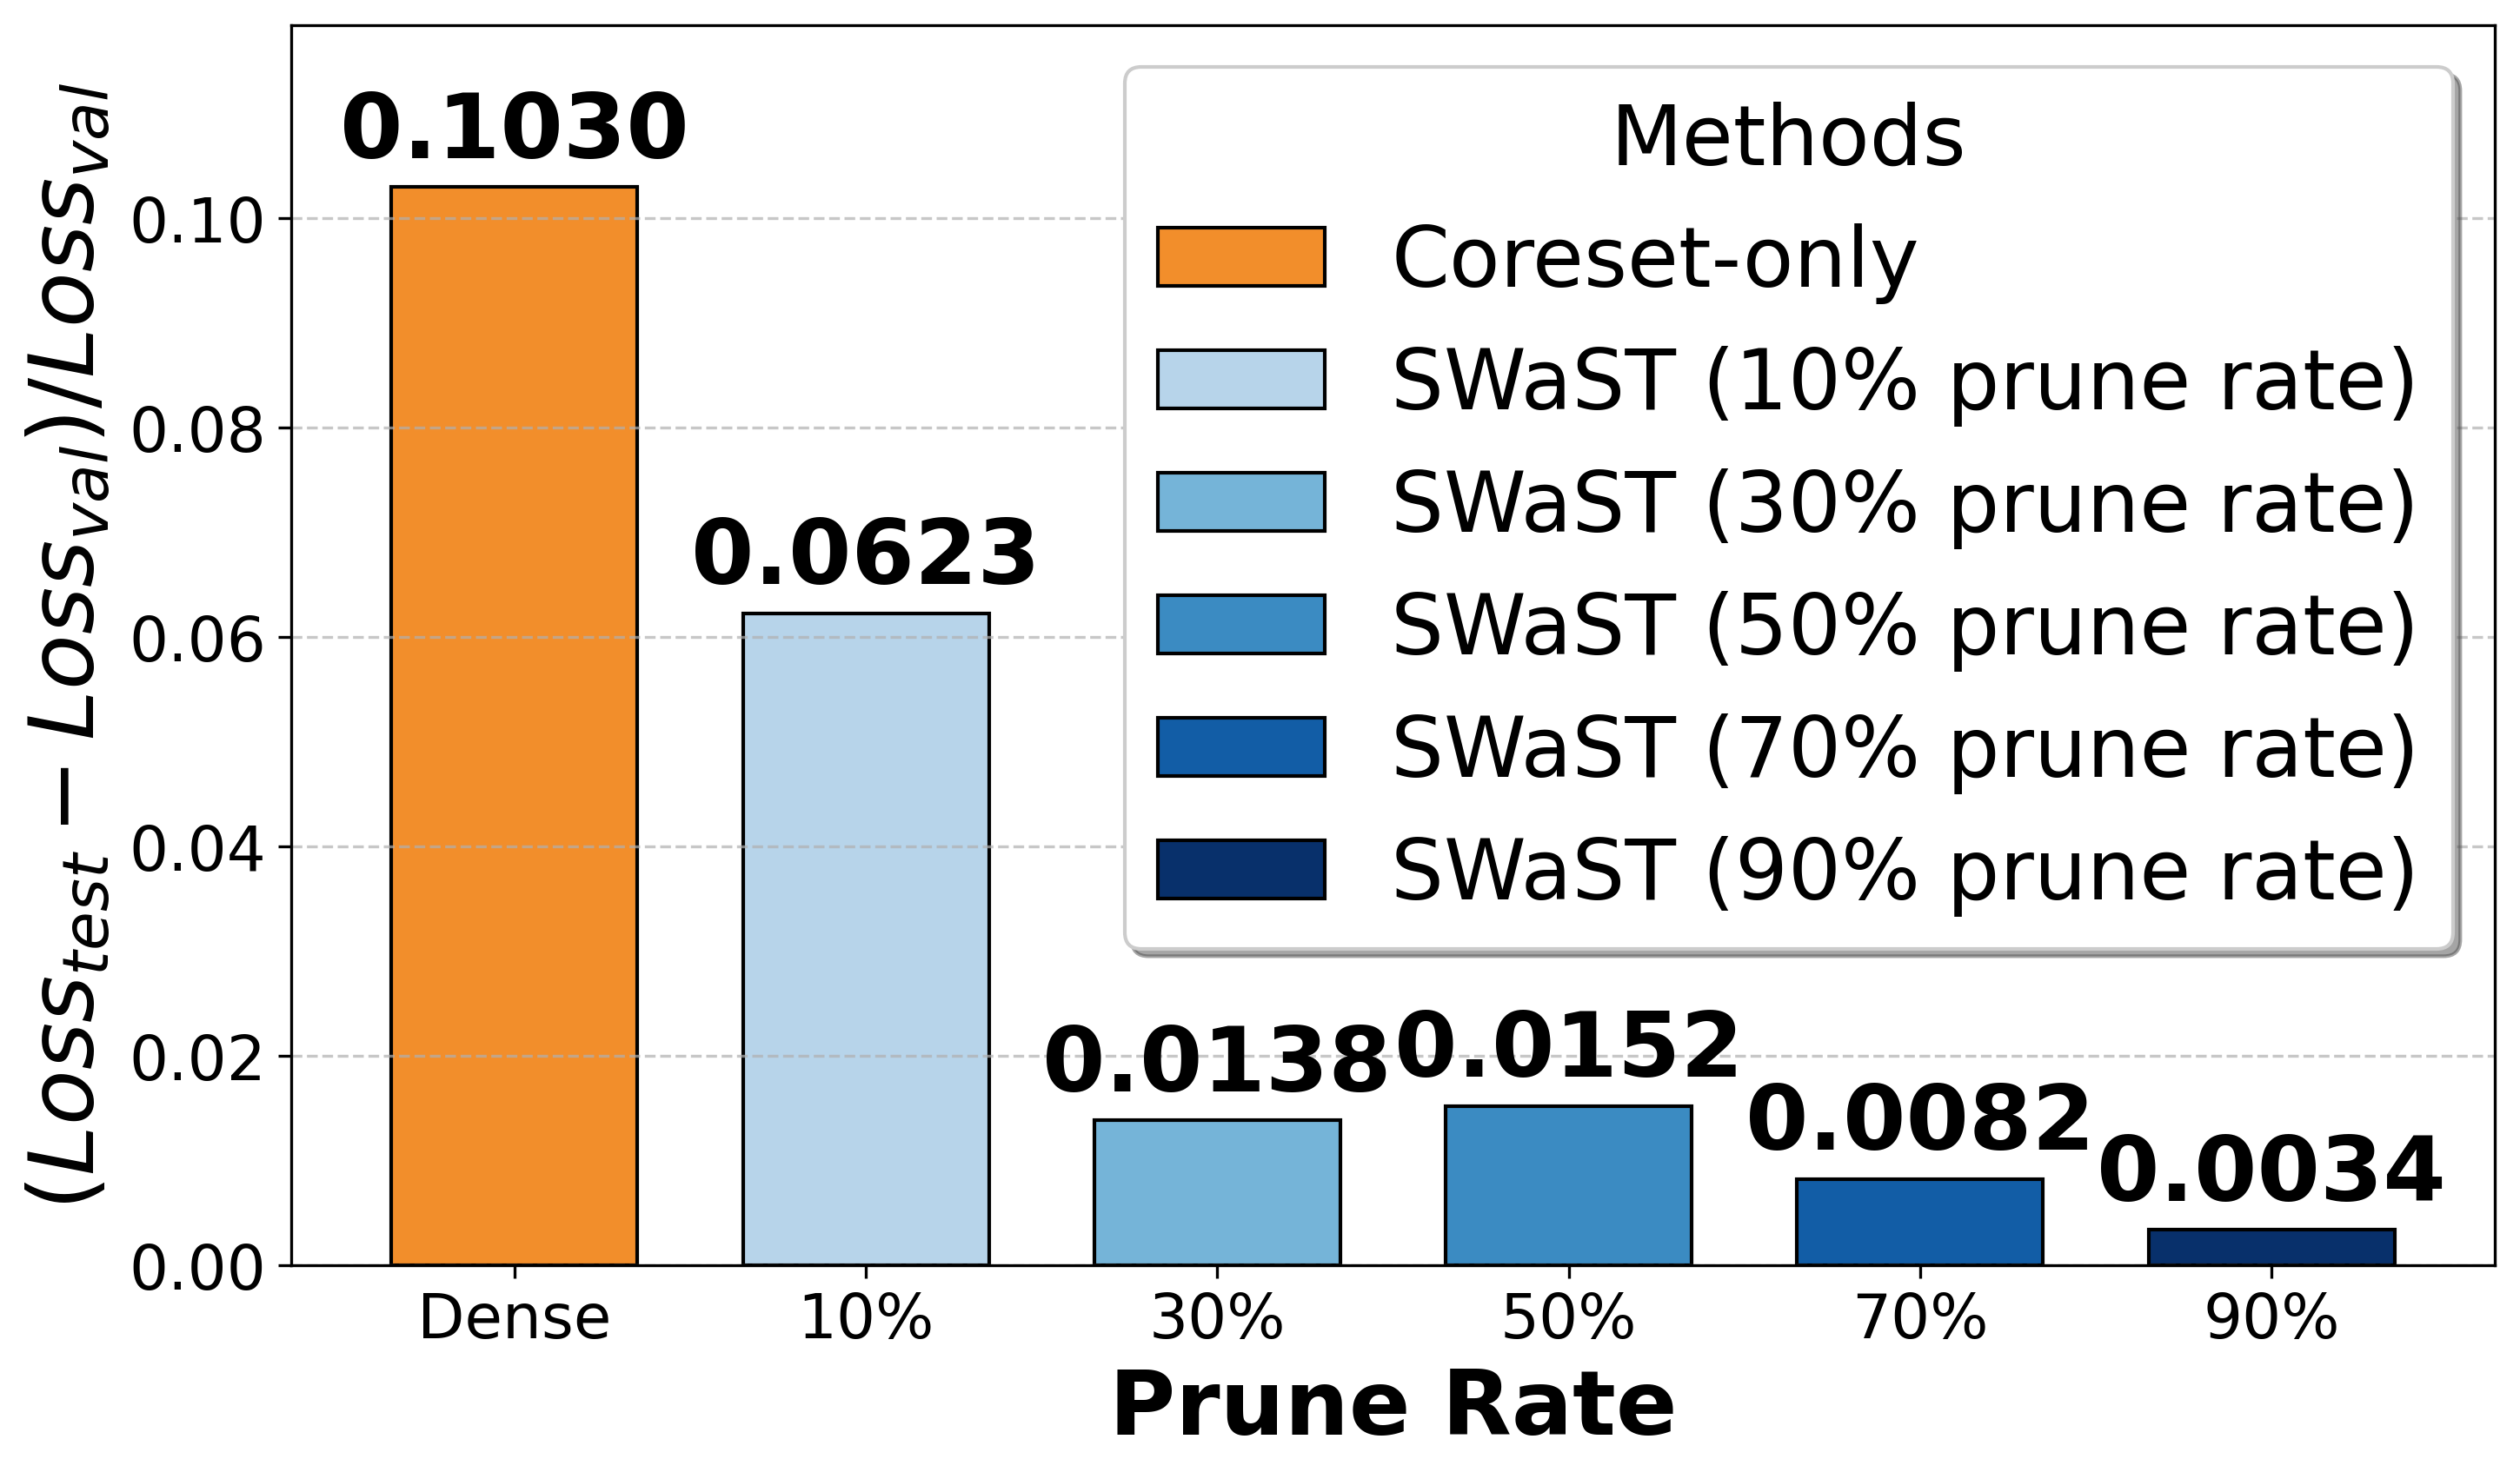
\includegraphics[width=1.0\linewidth]{figs/overfitting_comparison.png}
    \caption{Overfitting}
    \label{fig:overfitting}
  \end{subfigure}
  \hfill
  \begin{subfigure}{0.32\linewidth}
    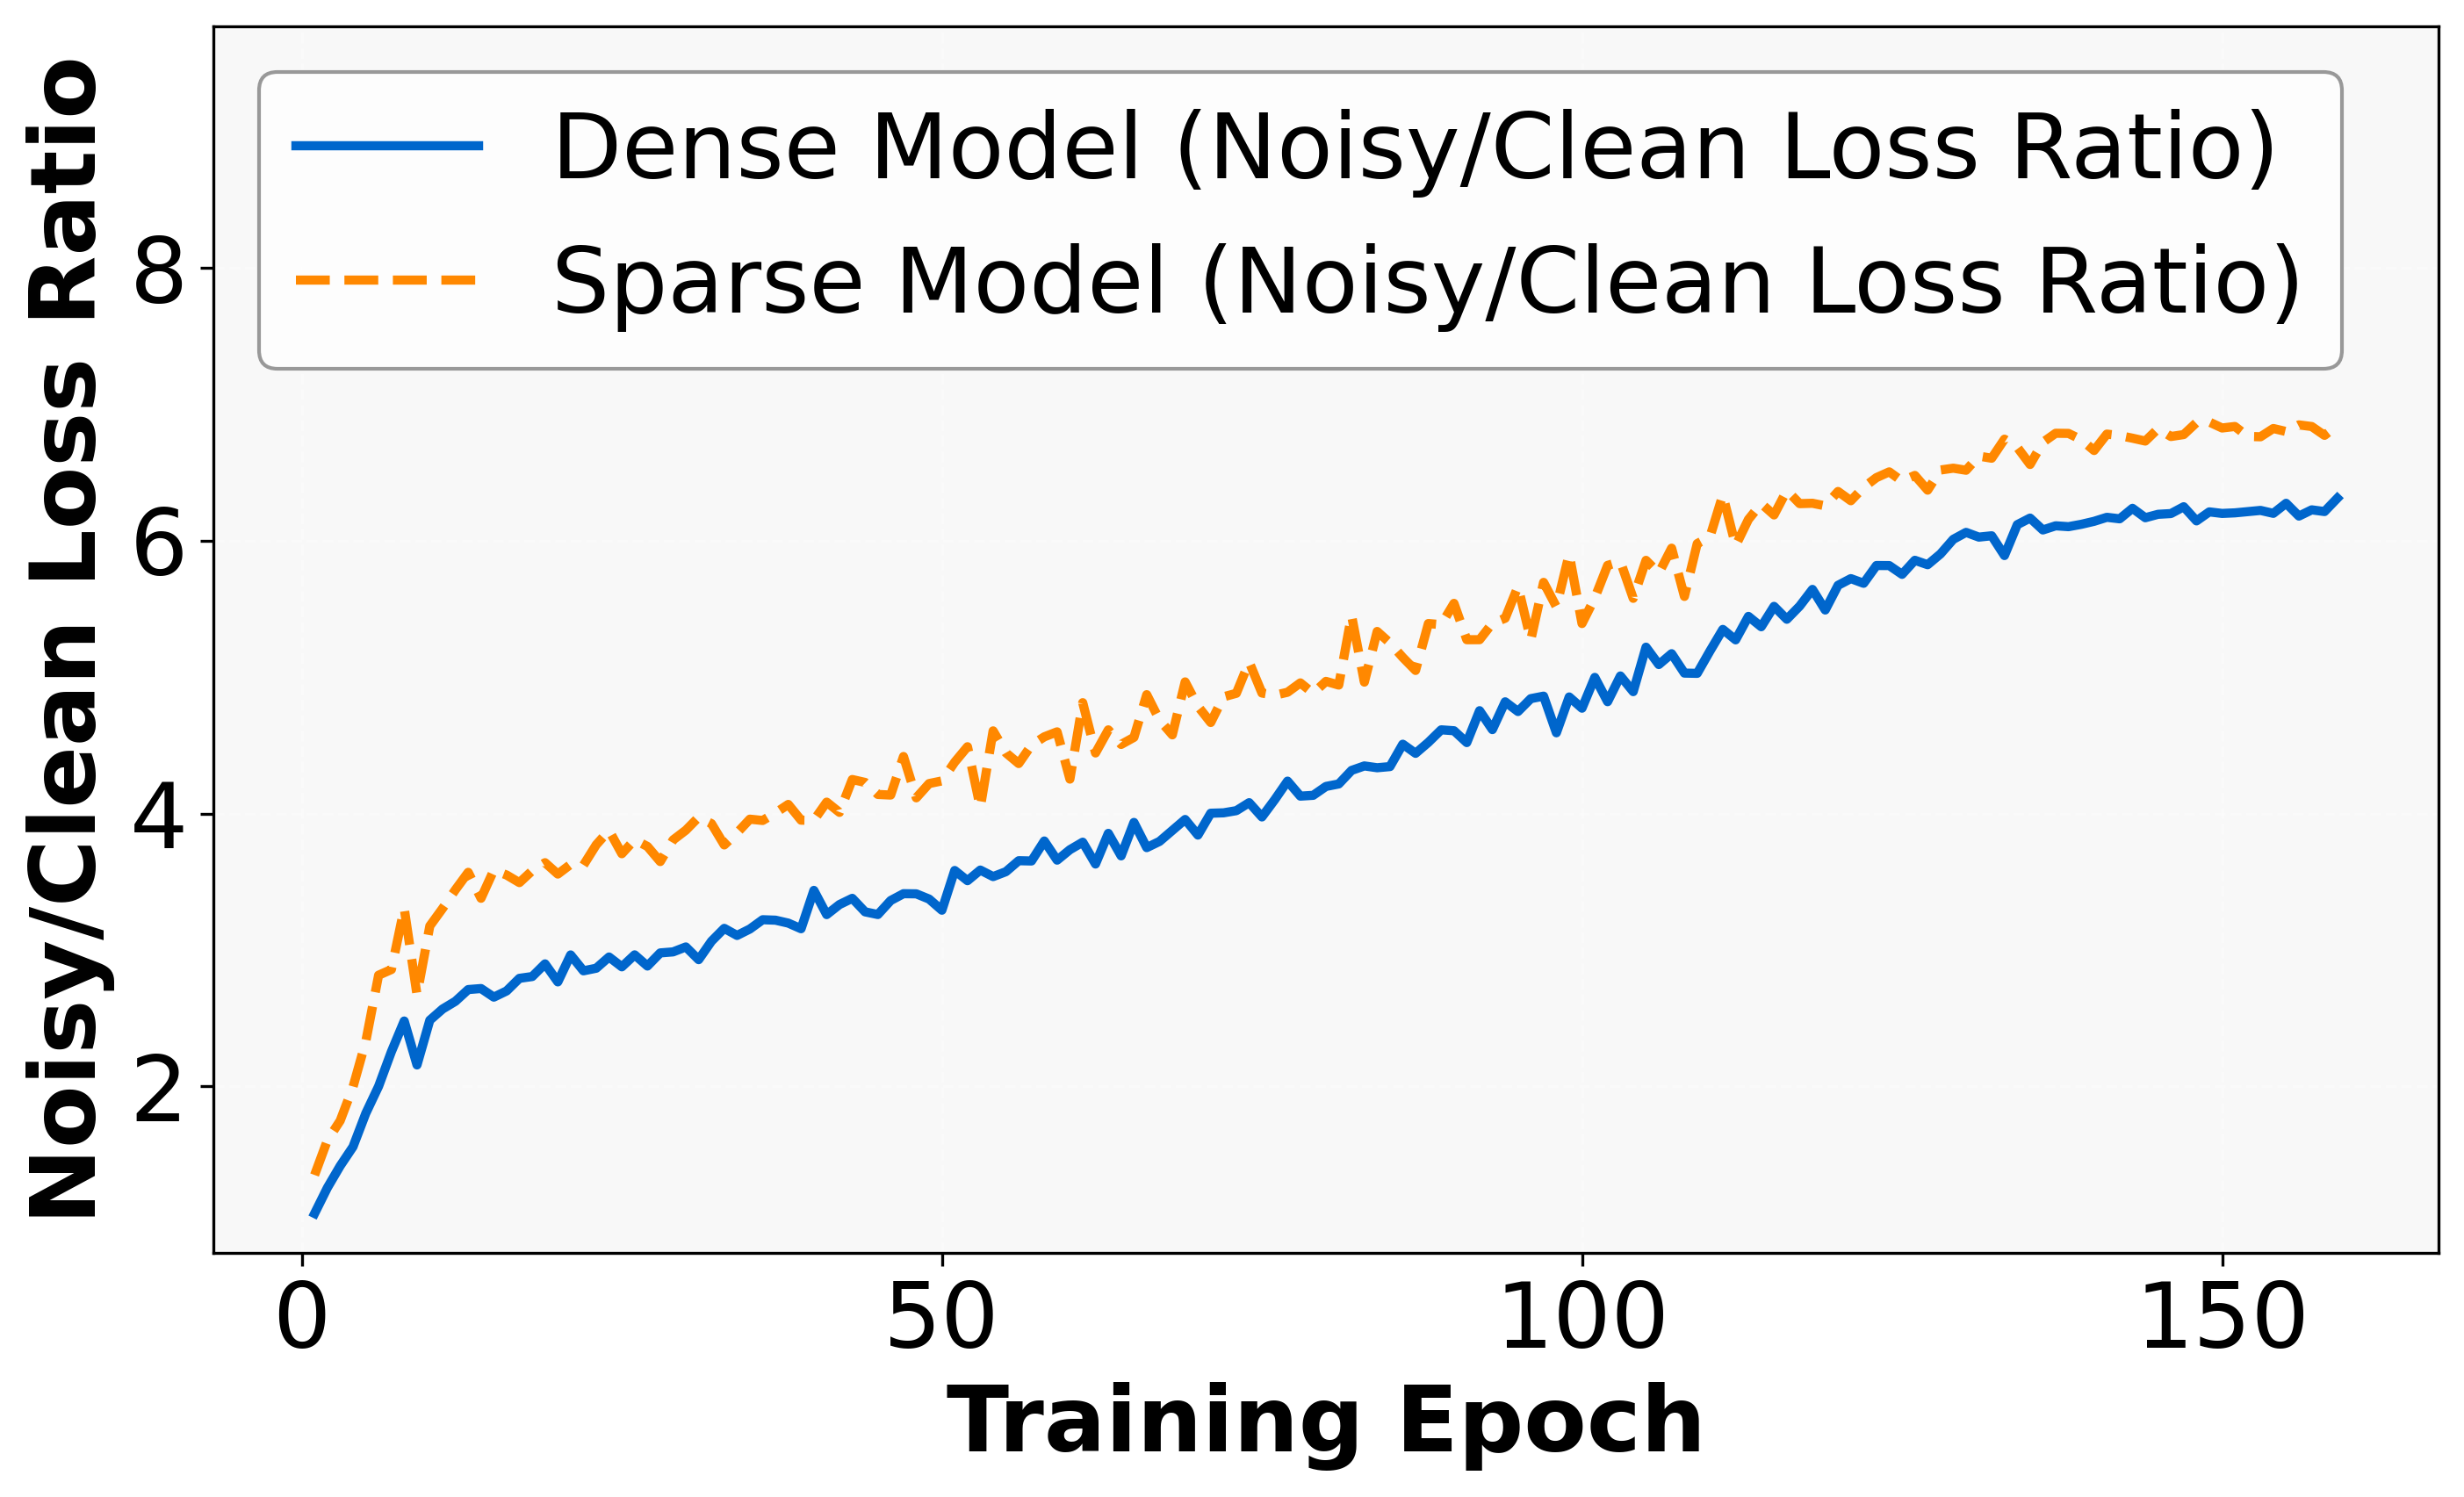
\includegraphics[width=1.0\linewidth]{figs/loss_comparison.png}
    \caption{Loss differences}
    \label{fig:noise_loss}
  \end{subfigure}
  \caption{Results demonstrating the effectiveness of SWaST (lower values are better in (a) and (b), higher values are better in (c)).  
  (a) Noise ratio in selected coresets across training rounds comparing SWaST to the coreset-only baseline, with a 10.62\% reduction in the final selection. 
  (b) Overfitting comparison measured by test loss minus validation loss. SWaST significantly reduces overfitting compared to the dense model (Coreset-only), with higher prune rates yielding progressively better overfitting reduction.
  (c) Loss ratio between noisy and clean samples during training, showing that weight pruning increases the loss on noisy samples while preserving performance on clean data.}  
\end{figure*}
\begin{itemize}
    \item \textbf{Row-wise analysis:} Both SWaST-trim and SWaST-cut consistently outperform the coreset-only baseline across all configurations, achieving accuracy improvements of up to 17.83\%.
    \item \textbf{Column-wise analysis:} The performance gains from SWaST become more pronounced as coreset size diminishes. This trend aligns with our intuition: smaller coresets present greater selection challenges, where weight pruning facilitates the identification of higher-quality samples (see Fig.~\ref{fig:noise_ratio} and~\ref{fig:noise_loss}). Simultaneously, reduced coreset sizes exacerbate overfitting, which pruning effectively mitigates (see Fig.~\ref{fig:overfitting}).
\end{itemize}
Additional experiments on noisy datasets corroborate these findings, showing consistent performance improvements across diverse data conditions (see Appendix).

\begin{figure}[!htbp]
  \centering
  \begin{subfigure}{0.49\linewidth}
    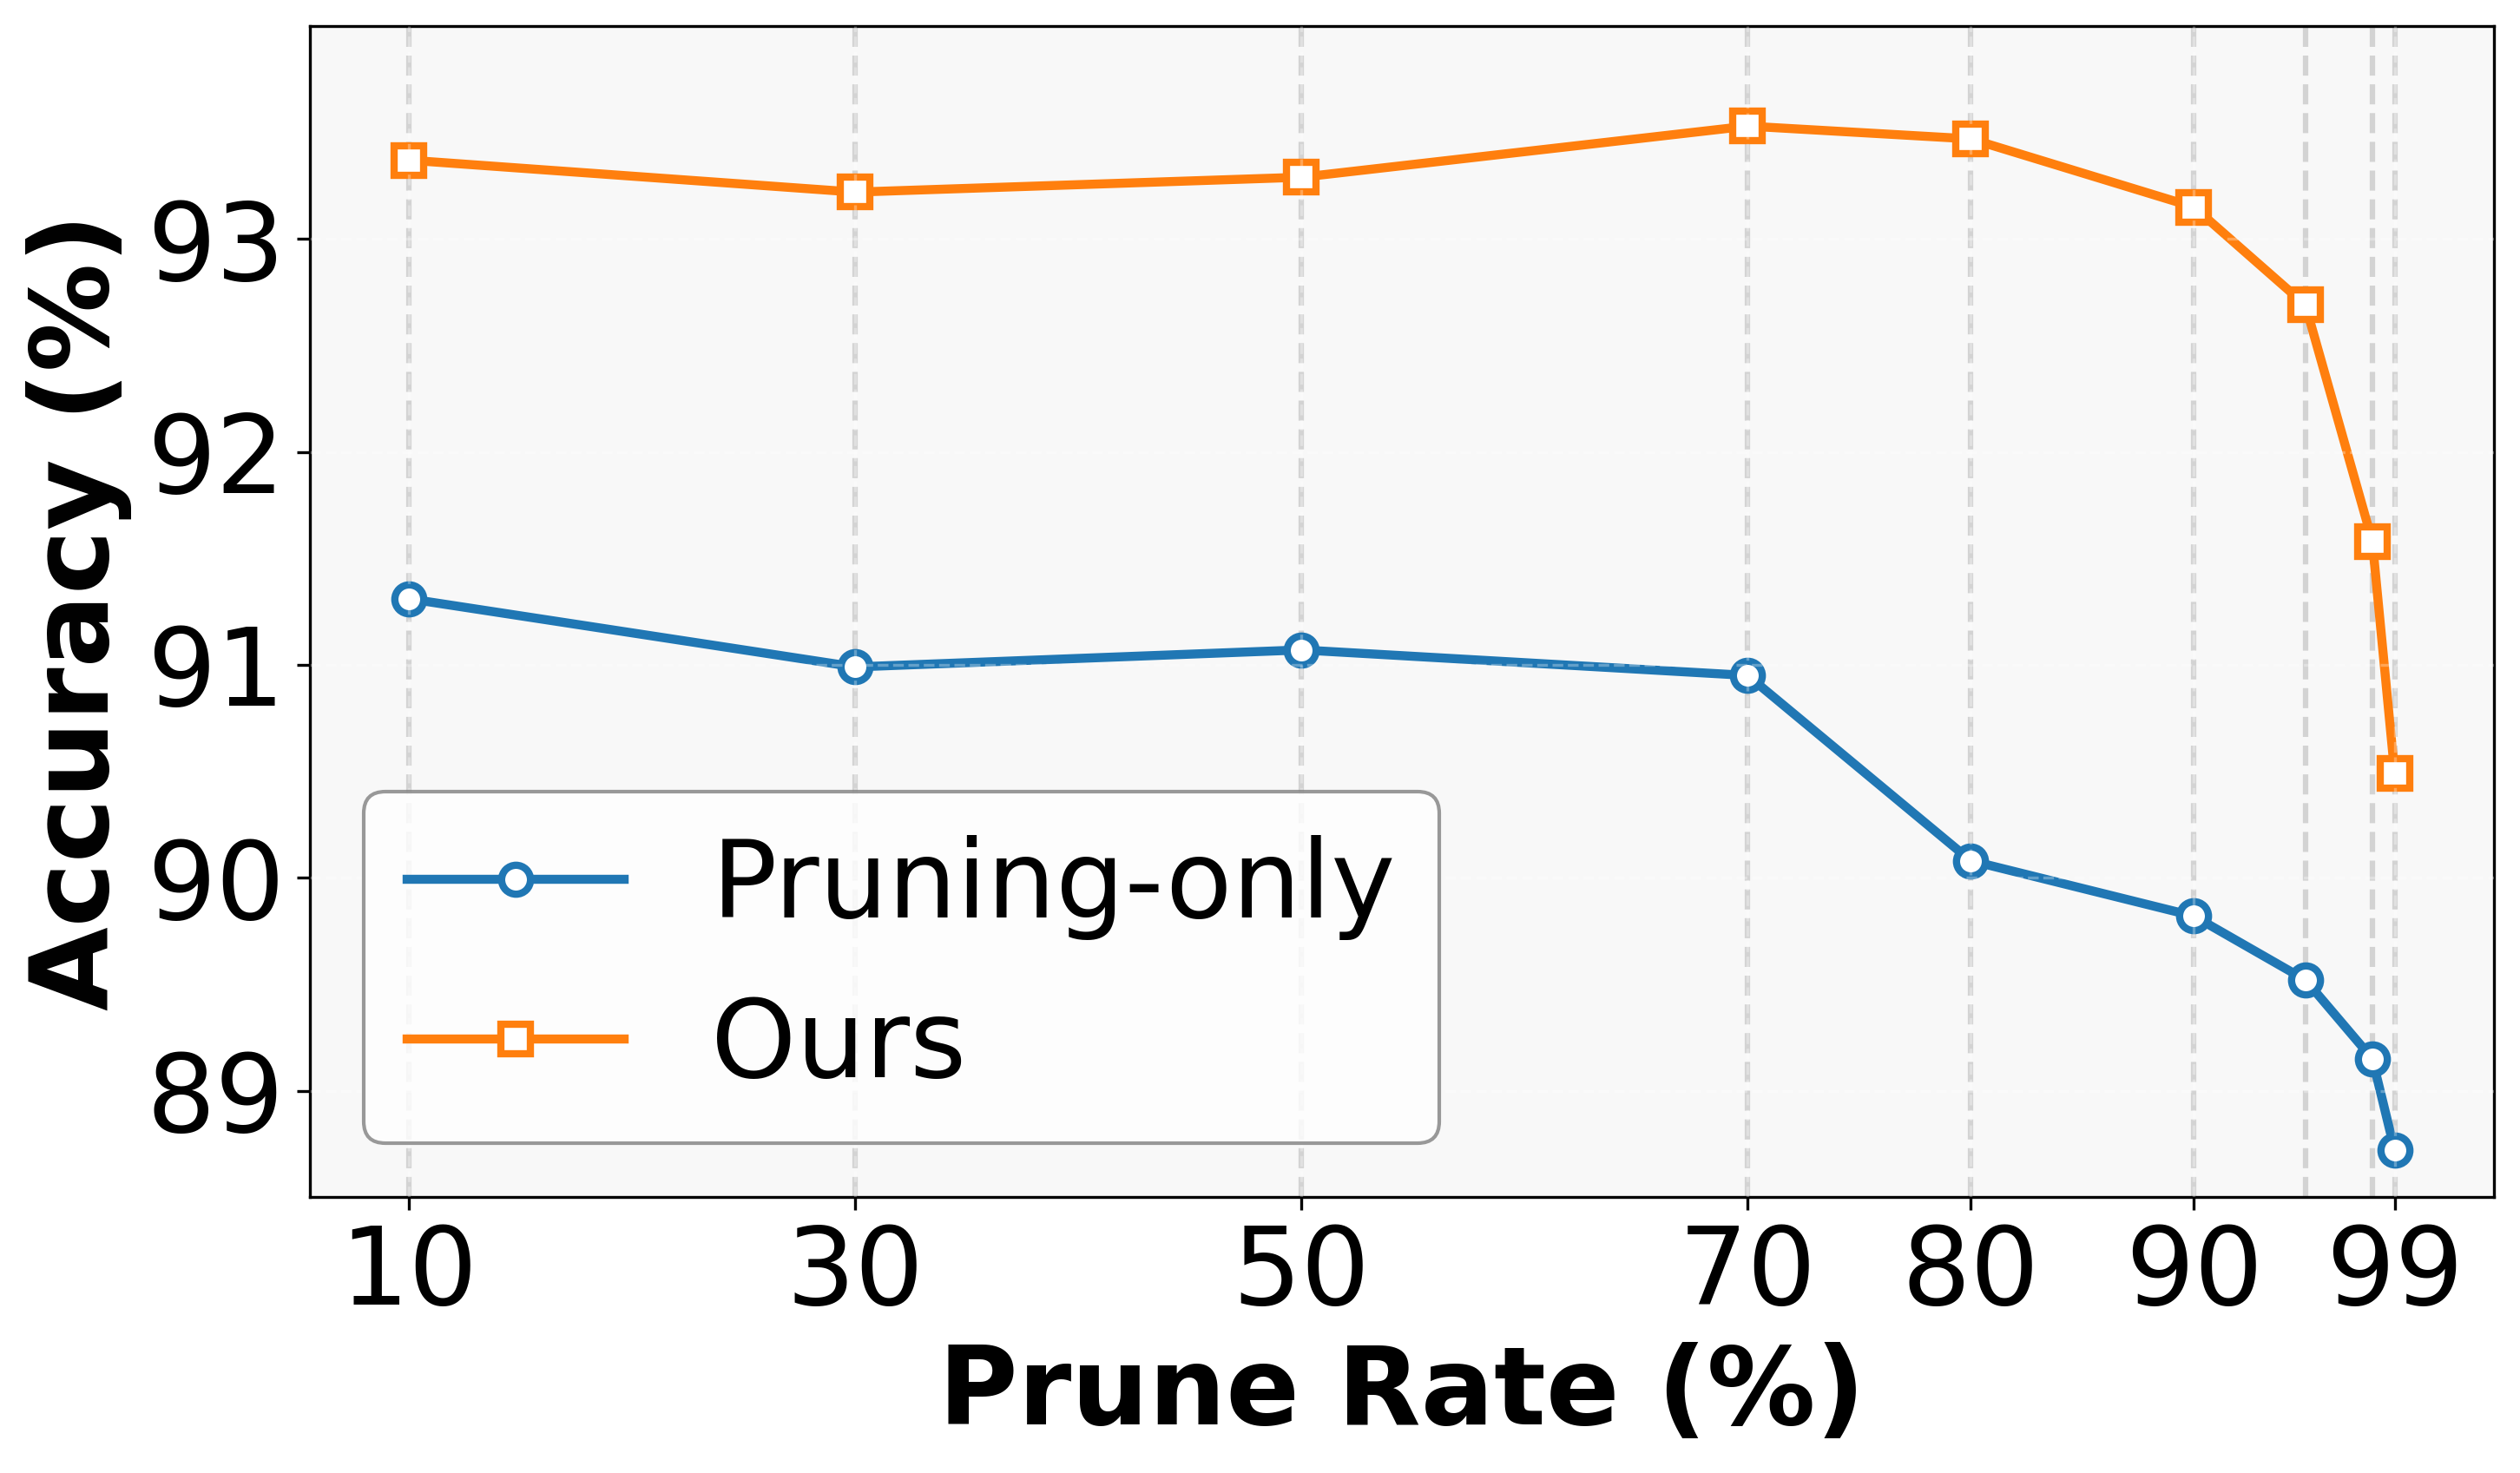
\includegraphics[width=1.0\linewidth]{figs/noise_prune.png}
    \caption{Accuracy vs. pruning rate}
    \label{fig:noise_prune}
  \end{subfigure}
  \hfill
  \begin{subfigure}{0.49\linewidth}
    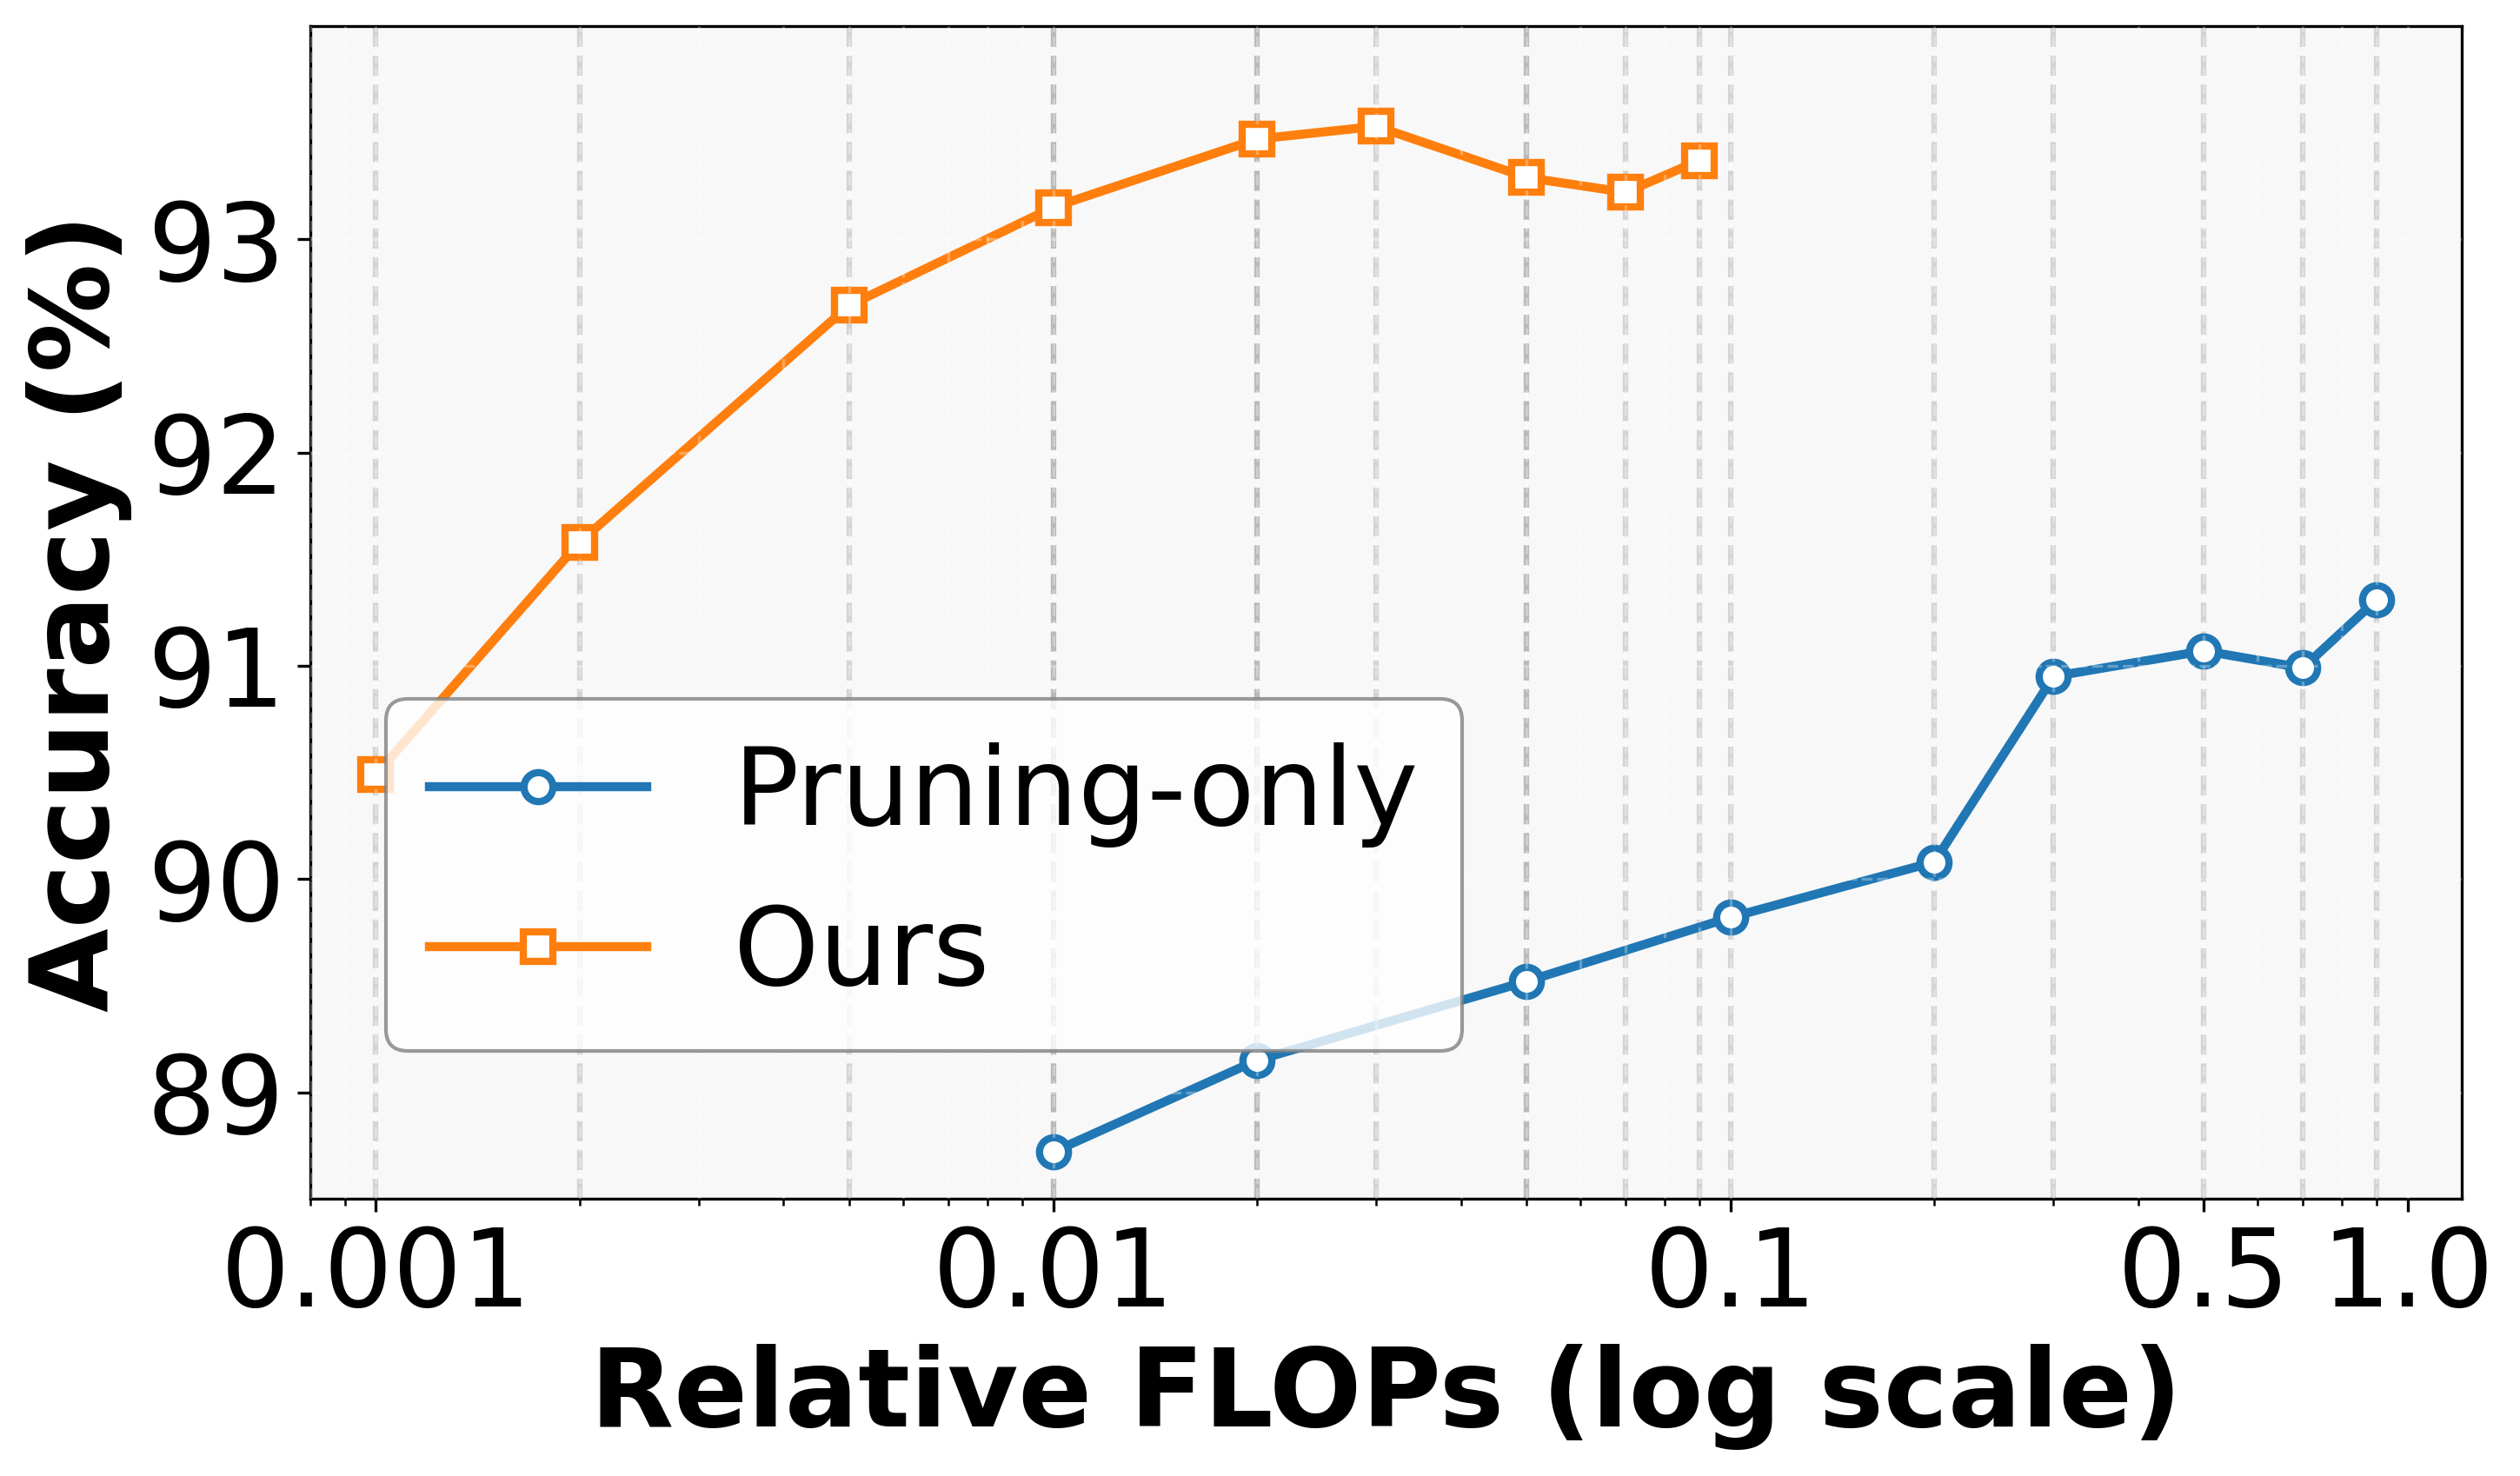
\includegraphics[width=1.0\linewidth]{figs/noise_prune_flops.png}
    \caption{Accuracy vs. FLOPs}
    \label{fig:noise_prune_flops} 
  \end{subfigure}
  \caption{Performance comparison between SWaST-cut and pruning-only baseline. (a) SWaST-cut achieves higher accuracy across different pruning rates, with more pronounced improvements at high sparsity levels. (b) Due to coreset selection, SWaST-cut demonstrates superior accuracy-efficiency trade-offs, significantly outperforming the baseline under equivalent computational budgets.}
\end{figure}

\paragraph{Coreset selection improves weight pruning.}
We adopt the coreset algorithm from \citep{xia2022moderate} to identify the most informative samples. As shown in Fig.~\ref{fig:noise_prune} and Fig.~\ref{fig:noise_prune_flops}, SWaST delivers two key benefits:
\begin{itemize}
  \item \textit{Higher accuracy}: SWaST achieves 93.15\% accuracy at a 90\% pruning rate—an improvement of 3.33\% over the pruning-only baseline.
  \item \textit{Better efficiency}: Benefiting from the reduced training overhead through coreset selection, SWaST achieves superior accuracy under comparable FLOPs budgets with a gap of up to 4.43\% when the relative FLOPs is 0.01.
\end{itemize}


